\selectlanguage{english}%

\chapter{Sistemas Fuzzy} \label{capFundFuzzy}
A lógica fuzzy, ou difusa, foi introduzida originalmente por Lofti A. Zadeh, em seu artigo "Fuzzy sets and systems" \cite{zadeh}. Sua teoria diverge da lógica booleana convencional no tratamento da pertinência das variáveis, podendo assumir qualquer valor entre todos os possíveis de um intervalo. Essa abordagem é mais eficaz na descrição de alguns sistemas reais, uma vez que é praticamente impossível eliminar todas as incertezas nos modelos que os representam. Este capítulo apresenta os fundamentos desse paradigma bem como sua aplicação na modelagem, proposta por Takagi e Sugeno \cite{takagiSugeno}.

\section{Conjuntos Fuzzy}
De acordo com a teoria de conjuntos clássica, um elemento $x$ qualquer, pode pertencer ou não à um conjunto universo de discurso $U$, ou seja $x \in U$ ou $x \notin U$ . Portanto, para qualquer conjunto determinado, pode-se estar completamento dentro ou completamente fora dele.

\begin{align}
	f_u(x) : U \rightarrow \{0,1\}
	&& f_u(x) =
	\begin{cases*}
		1 & se e somente se $x \in U$ \\
		0 & caso contrário
	\end{cases*}
	\label{eqFPertinencia}
\end{align}

Essa definição binária se encaixa bem em problemas restritos, cujo caráter dos sistemas reflita essa separação clara de estados, por exemplo a paridade ou não de uma da soma dos bits de uma mensagem binária. Conhecendo-se os valores, este resulte é ímpar ou par, indubitavelmente. No entanto, grande parte dos sistemas estudados nas teorias de controle trabalha com grandezas que não possuem limites tão claros assim, como exemplo a sensação térmica. Apesar de a temperatura ser matematicamente bem definida, existem descrições como "frio" e "quente" que não podem ser representadas com este conjunto binário, uma vez que são conceitos vagos e imprecisos.

A abordagem fuzzy aparece como uma alternativa muito capaz de tratar estes casos. Seus conjuntos são caracterizados por uma função contínua de pertinência fuzzy, que relaciona cada elemento do universo de discurso à sua conformidade no conjunto, podendo abranger todos os valores no intervalo de pertinência.

\subsection{Variáveis Linguísticas}
As variáveis linguísticas são os termos que constituem os conjuntos nebulosos. Tratam-se de traduções das variáveis reais na forma de valores linguísticos, não numéricos. Assim, seguindo com exemplo anterior, a temperatura seria a variável linguística e "quente", "frio", "muito quente" e "muito frio" alguns de seus possíveis valores linguísticos. Estes últimos são os conjuntos difusos e possuem, cada um deles, uma função de pertinência mapeando a adequação de uma determinada temperatura a sua conformidade neles.

\section{Funções de Pertinência}
\label{secFncPert}
O conceito chave de toda a abordagem fuzzy são as funções de pertinência. Em exemplo, dados os conjuntos fuzzy $U_1$, $U_2$ e $U_3$, cada qual possui sua função de pertinência $f_1(x)$, $f_2(x)$ e $f_3(x)$, para todo elemento pertencente ao universo de discurso.

\begin{align}
	f_i(x) : i \rightarrow [0,1]
	\label{eqFuncPertFuzzy}
\end{align}
Onde $f_i(x)=0$ implica que o elemento $x$ é "completamente não" $U_i$ e $f_i(x)=1$ indica que $x$ é "completamente" $U_i$. Mas, diferentemente da lógica convencional, é possível que um elemento seja 50\% pertinente à $U_1$ ($f_1(x)=0.5$), 30\%  à $U_2$ ($f_2(x)=0.3$) e 20\%  à $U_3$ ($f_3(x)=0.2$).

Apesar de operar sobre grandezas linguísticas, é importante notar que normalmente os elementos são variáveis numéricas, portanto as funções de pertinência precisam ser bem definidas no intervalo do conjunto. Os formatos mais comuns para elas são apresentados na \hyperref[figPert]{Figura \ref{figPert}} a seguir:

\begin{figure}[H]
	\centering
\begin{tabular}{ccc}
	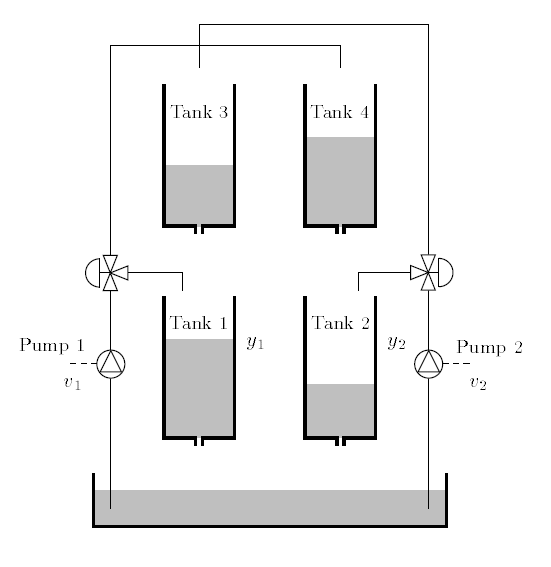
\includegraphics[width=0.3\textwidth,keepaspectratio]{img/4tank.png} &
	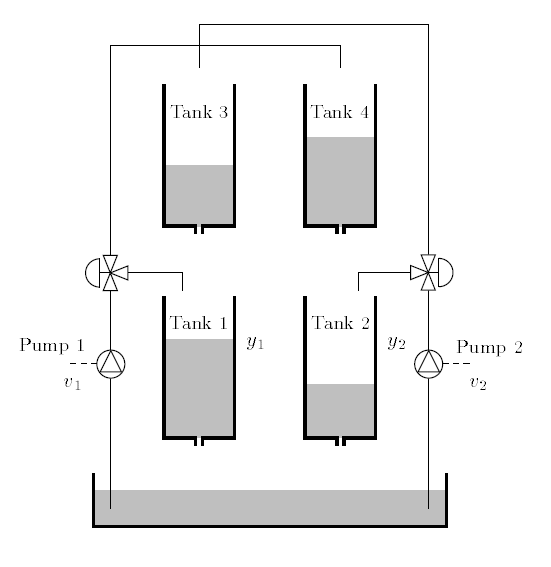
\includegraphics[width=0.3\textwidth,keepaspectratio]{img/4tank.png} &
	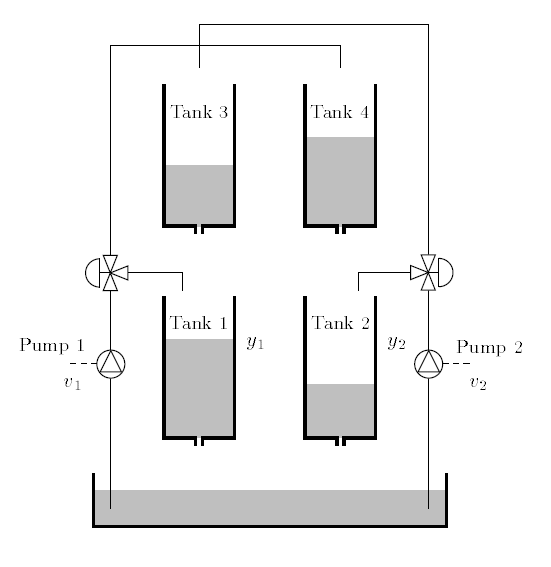
\includegraphics[width=0.3\textwidth,keepaspectratio]{img/4tank.png} \\
	(a) Triangular &
	(b) Senoidal
	(c) Trapezoidal \\
	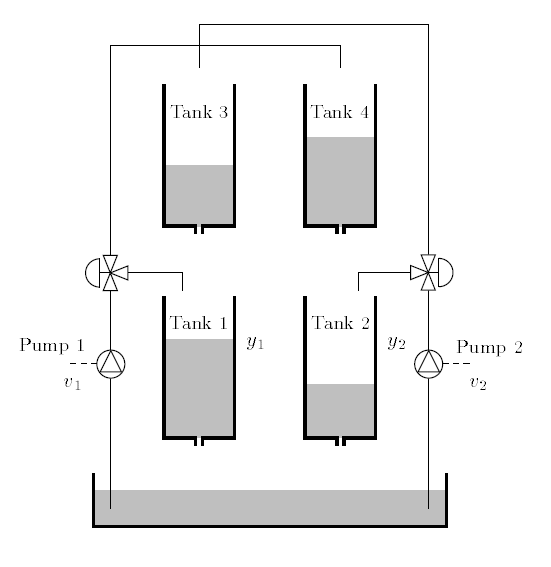
\includegraphics[width=0.3\textwidth,keepaspectratio]{img/4tank.png} &
	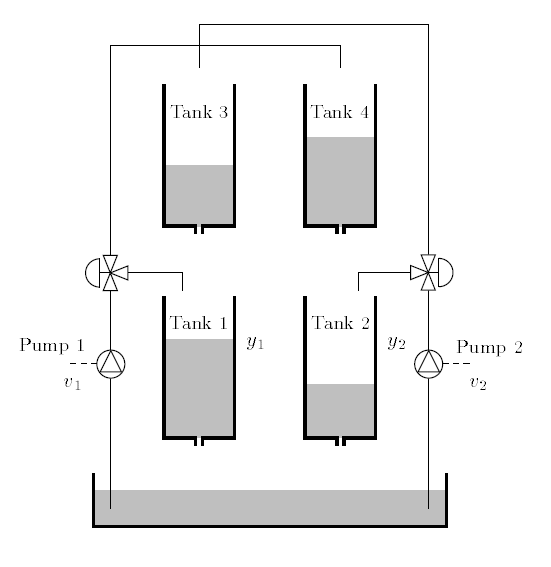
\includegraphics[width=0.3\textwidth,keepaspectratio]{img/4tank.png} &
	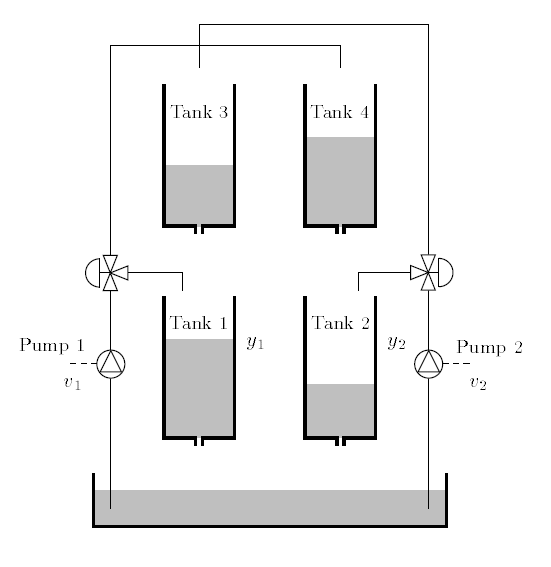
\includegraphics[width=0.3\textwidth,keepaspectratio]{img/4tank.png} \\
	(d) Gaussiana &
	(e) Sigmoide &
	(f) Quadrada
\end{tabular}
	\caption{\label{figPert}Funcões de Pertinência.}
\end{figure}

Apresenta-se a seguir os procedimentos comuns para obtenção da função de pertinência de um dado sistema, ilustrando-se com o exemplo:
\begin{itemize}
	\item \textbf{Definir a variável linguística:} "Temperatura"
	\item \textbf{Definir os conjuntos fuzzy:} \{"muito frio"\}, \{"frio"\}, \{"quente"\}, \{"muito quente"\}
	\item \textbf{Definir os limites de cada conjunto:} $[-10ºC,5ºC]$,$ [5ºC,15ºC]$, $[15ºC,30ºC]$, $[30ºC,45ºC]$ 
	\item \textbf{Definir as funções de pertinência:} Neste caso opta-se por funções triangulares, com picos nos centros dos intervalos e nulas em qualquer caso fora deles.
\end{itemize}

Os resultados do exemplo são apresentados na \jhhref{figPertEx}{Figura} a seguir:
\begin{figure}[H]
	\centering
	\begin{tabular}{cc}
		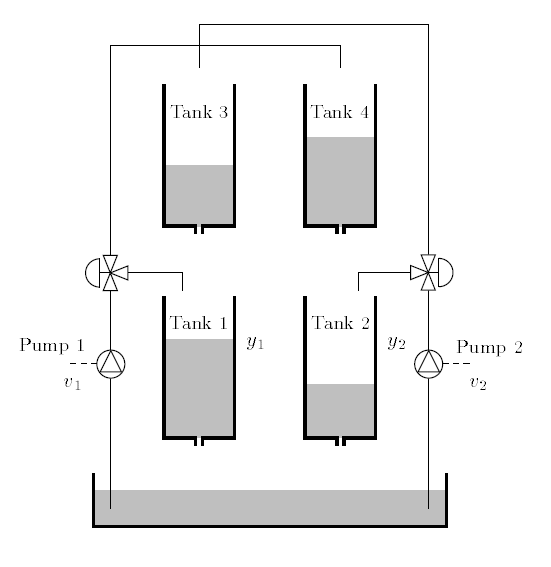
\includegraphics[width=0.3\textwidth,keepaspectratio]{img/4tank.png} &
		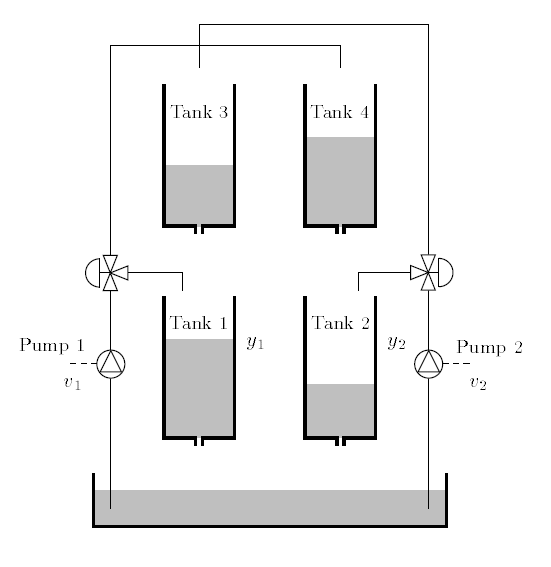
\includegraphics[width=0.3\textwidth,keepaspectratio]{img/4tank.png} \\
		(a) Pertinência do conjunto "muito frio" &
		(b) Pertinência do conjunto "frio" \\
		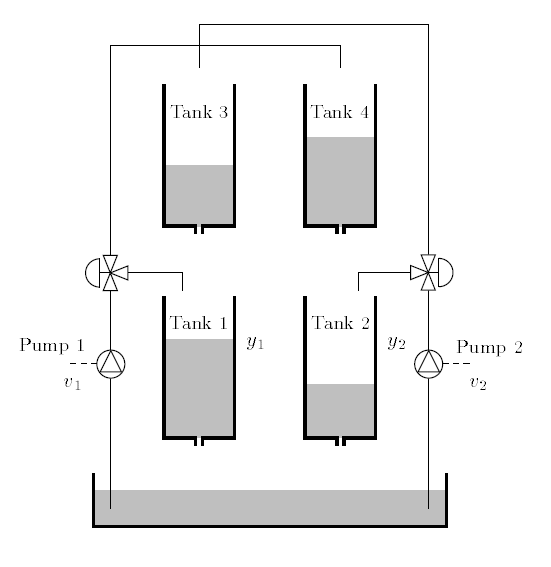
\includegraphics[width=0.3\textwidth,keepaspectratio]{img/4tank.png} &
		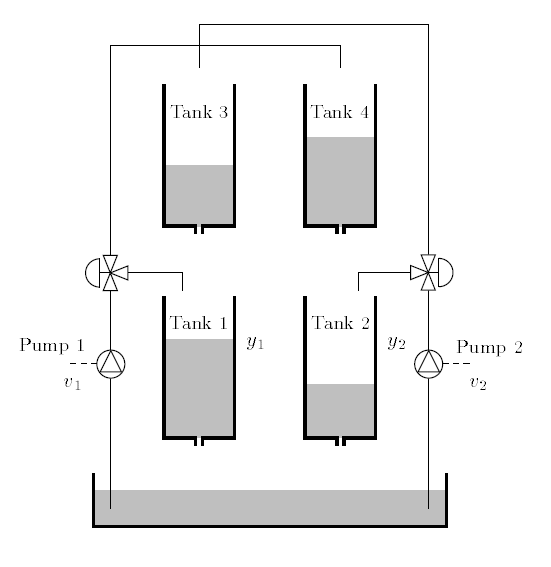
\includegraphics[width=0.3\textwidth,keepaspectratio]{img/4tank.png} \\
		(c) Pertinência do conjunto "quente" &
		(d) Pertinência do conjunto "muito quente"
	\end{tabular}
	\caption{\label{figPertEx} Funções de Pertinência.}
\end{figure}	

A \jhhref{tabPertEx}{Tabela} a seguir apresenta os graus de pertinência de várias amostras a cada conjunto:

\begin{table}[!ht]
	\caption{Tabela de Exemplos}
	\label{tabPertEx}
	\small
	\centering
	\scalebox{1}{
		\begin{tabular}{|c|c|c|c|c|}
			\hline
			Temperatura & Muito Frio & Frio & Quente & Muito Quente \\
			\hline
			0 & 0 & 0 & 0 & 0 \\
			\hline
			0 & 0 & 0 & 0 & 0 \\
			\hline
			0 & 0 & 0 & 0 & 0 \\
			\hline
			0 & 0 & 0 & 0 & 0 \\
			\hline
			0 & 0 & 0 & 0 & 0 \\
			\hline
			0 & 0 & 0 & 0 & 0 \\
			\hline
			0 & 0 & 0 & 0 & 0 \\
			\hline
			0 & 0 & 0 & 0 & 0 \\
			\hline
		\end{tabular}
	}
\end{table}

É importante notar que a soma final dos valores de todas as pertinências de um elemento precisa ser 1, para que haja coerência entre o modelo e o real.

\section{Aplicação}
A aplicação da lógica fuzzy na teoria de controle se dá através da utilização de regras que definem o modelo final baseando-se no grau de pertinência do estado do sistema a cada um dos conjuntos difusos. 

De maneira similar à tradicional, a lógica fuzzy baseia-se no paradigma de implicações, ou \textit{modus ponens}. Esta linha de raciocínio é organizada em regras que implicam em conclusões a partir da autenticidade de premissas. O \jhhref{eqRegrasEx}{exemplo} a seguir ilustra:

\begin{align} \label{eqRegrasEx}
\begin{cases}
	\text{(1) Se está  chovendo então é perigoso dirigir}\\
	\text{(2) Está chovendo }\\
	\text{(3) É perigoso dirigir}
\end{cases}		
\end{align}

A afirmação (1) é chamada de regra de implicação, ou regra Se-Então, e é ela quem rege o comportamento da conclusão (3) de acordo com a premissa (2). 

\subsection{Regras Se-Então}
Como visto no \jhhref{eqRegrasEx}{exemplo} as regras Se-Então são as premissas que definem os resultados das afirmações. Na teoria fuzzy faz-se uso das funções de pertinência para decidir as conclusões. Assim, ao contrário da lógica clássica onde há ou não ativação de uma determinada regra, em lógica difusa toda regra está ativada em determinado grau. Exemplifica-se a seguir:

\begin{align*} \label{eqRegraDef}
\text{Regra: }
\begin{cases}
	\text{SE: X pertence a A} \\
	\text{ENTÃO: Y pertence a B}
\end{cases}		
\end{align*}

O grau de ativação da Regra na \jhhref{eqRegraDef}{equação} é definido a partir da pertinência do elemento $X$ em $A$. A conclusão $Y$ será definida de forma a cumprir pertinência semelhante ao conjunto $B$.

Prosseguindo o exemplo inicial, pode-se utilizar a temperatura de uma sala para controlar a potência ativa de um ar condicionado. Define-se então conjuntos para a variável linguística "Potência": \{"muito fraca", "fraca", "forte", "muito forte"\}. 

\section{Modelo Fuzzy Takagi-Sugeno} \label{secTakSug}
Os trabalhos de Takagi, Sugeno \cite{takagiSugeno} e Kang \cite{kang}

\textbf{Regra i:}
\begin{align}
&\textbf{SE:} \text{ $v_1(t)$ é $M_{1i}$ e $v_2(t)$ é $M_{2i}$ e ... e $v_n(t)$ e $M_{ni}$,} \\
&\textbf{ENTÃO}: \ \ \begin{cases}
\dot{x}(t) = A_ix(t) + B_iu(t),\\
y(t) = C_ix(t)
\end{cases}
\label{eqRegraIGeral}
\end{align}


	\begin{equation}
	\begin{aligned}
		w_{1}(t) = M_1(h_1(t)) * N_1(h_2(t)) \\
		w_{2}(t) = M_1(h_1(t)) * N_2(h_2(t)) \\
		w_{3}(t) = M_2(h_1(t)) * N_1(h_2(t)) \\
		w_{4}(t) = M_2(h_1(t)) * N_2(h_2(t))
	\end{aligned}
	\end{equation}
	
	\begin{align}
		\dot{h}(t) = \frac{\sum_{i=1}^{4}  w_i(h(t))(A_i \Delta h_i(t) +  B_i \Delta u_i(t))}{\sum_{i=1}^{4} w_i(h)}
	\end{align}

Na concepção fuzzy, a regra Se-Então é disparada quando houver um grau de similaridade
não nulo entre a variável premissa e o antecedente. Como resultado, infere-se uma conclusão
que mantenha algum grau de similaridade com o conseqüente da regra. Nota-se, mais uma
vez, que os conceitos tradicionais estão embutidos na teoria fuzzy. Se a variável premissa x
possui total similaridade com o antecedente A então a conclusão será que y é o próprio B.
Uma regra fuzzy pode possuir mais de um antecedente. Um exemplo simples é dado a
seguir:
R :
Se x é A e z é C
Então y é B
(2.5)
Neste caso, a maneira de inferir uma conclusão é bem mais elaborada. A conclusão depende
tanto da similaridade de x em A, quanto da similaridade de z em C. Além disso, depende da
relação entre ambos antecedentes, bem como da relação deles com o conseqüente.
Por exemplo, considere um veículo trafegando em uma estrada. Uma regra com múltiplos
antecedentes para inferir sobre a velocidade adequada do carro pode ser: “se a curva é fechada
ou a pista está molhada, então dirija em baixa velocidade”.
No caso de pista seca, quanto mais fechada for a curva, menor deve ser a velocidade.
Em outras palavras, quanto maior for a pertinência da variável “curva” no conjunto fuzzy
“fechada”, maior deverá ser a pertinência da “velocidade” no conjunto “baixa”.
Se o carro viaja pela mesma curva porém com pista molhada, por questão de segurança,
a velocidade deverá ser ainda menor. Neste caso a pertinência da “velocidade” no conjunto
“baixa” será afetada também pelo valor lingüístico da variável “pista”.
Existem diversas configurações que definem como os antecedentes interagem entre si e
com o conseqüente da regra para produzir uma conclusão. Tais configurações são chamadas
mecanismos de inferência e podem ser vistos com maiores

\indent A Teoria Fuzzy tem seu princípio cunhado por \cite{zadeh65}. Os trabalhos seguintes, como o \cite{takagi_sugeno} abordaram sua utilização para a modelagem de sistemas complexos por meio de aproximações, utilizando uma teoria de conjuntos diferente da convencional.

\subsection{Conjuntos Fuzzy}
\indent A teoria de conjuntos convencional utiliza lógica booleana para definir os valores lógicos das funções de pertinências dos conjuntos. Assim, dado $X$ o universo de discurso de um determinado conjunto $C$, um elemento genérico $x$ tem sua função de pertinência ao conjunto $C$ dado por:

\begin{align*}
f_{C}(x)&:X \rightarrow \{0,1\} \quad \\
f_{C}(x)&= 
\begin{cases}
1 \text{ se e somente se x} \in C \\
0 \text{ se e somente se x} \notin C\\
\end{cases}
\end{align*}

Existem, no entanto, situações em que a definição dos conjuntos de seus limites se tornam muito subjetivos. Nestas situações, a utilização da lógica difusa apresenta vantagens para a modelagem de sistemas. 

Considere-se como exemplo a temperatura de uma sala. Pode-se definir dois conjuntos de estados \{quente,frio\}. No entanto, torna-se um pouco confuso e arbitrário decidir em qual destes conjuntos um estado específico se encaixa. Utilizando funções de pertinências não binárias, observa-se o \textbf{quanto} determinada temperatura se encaixa em cada um dos conjuntos. Funções de pertinências fuzzy são definidas da forma:

\begin{align*}
f_{C}(x)&:X \rightarrow [0,1]
\end{align*}

\subsection{Funções De Pertinência}
Existem várias normas e regras disponíveis para funções de pertinência. Este trabalho considera a norma triangular. Seguindo o exemplo dado, dada uma temperatura $x$ verifica-se o quão pertencente aos conjuntos \textit{quente} e \textit{fria} ela é utilizando a função do gráfico a seguir:

\begin{figure}[H]
	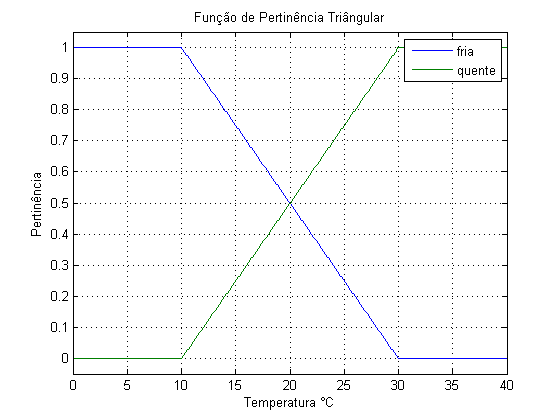
\includegraphics[width=0.5\textwidth]{img/pertinencia.png}
	\caption{Diagrama esquemático do sistema de quatro tanques e planta didática.}
	\label{figPertinencia}
\end{figure}

Nota-se que se escolhem limites para os conjuntos: toda temperatura abaixo de 10 é fria; toda temperatura acima de 30 é quente. As demais, pertencem mais ou menos à cada um dos conjuntos.

Em lógica Fuzzy, as variáveis definidas de forma subjetiva, com expressões para limites são chamadas variáveis linguísticas.




\selectlanguage{brazil}%

